\documentclass{article}[18pt]
\usepackage{../../../format}
\lhead{A Level Physics - Fields}

%File specific Preamble
\usetikzlibrary{decorations, decorations.text,positioning,quotes,arrows.meta,decorations.markings,3d,shapes,decorations.pathmorphing,calc,quotes,angles}
\usepackage[super]{nth}
\tikzstyle{arrow} = [thick,->,>=stealth]

\pgfkeys{/pgfplots/Axis Style/.style={
    width=7cm, height=5cm,
    axis x line=center, 
    axis y line=middle, 
    samples=300,
    ymin=-1, ymax=1,
    xmin=0, xmax=4,
    domain=-4*pi:4*pi
}}

\pgfkeys{/pgfplots/Axis Style 2/.style={
    width=13.5cm, height=8cm,
    axis x line=center, 
    axis y line=middle, 
    samples=200,
    ymin=-1, ymax=1,
    xmin=0, xmax=6.5,
    domain=-4*pi:2*pi
}}

\pgfkeys{/pgfplots/Axis Style 3/.style={
    width=7cm, height=5cm,
    axis x line=center, 
    axis y line=middle, 
    samples=200,
    ymin=-1.5, ymax=1.5,
    xmin=0, xmax=14.0,
    domain=-4*pi:4*pi
}}

\begin{document}
\begin{center}
\underline{\huge Electromagnetic Induction}
\end{center}
\section{Generating Electricity}
$ $\\
$ $\\

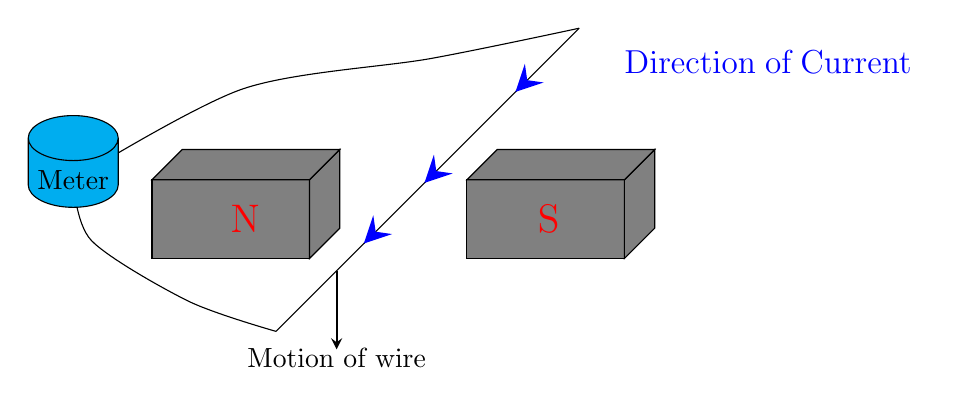
\begin{tikzpicture}
\tikzset{myptr/.style={decoration={markings,mark=at position 1 with %
    {\arrow[scale=3,>=stealth,blue]{>}}},postaction={decorate}}}
\pgfmathsetmacro{\cubex}{2}
\pgfmathsetmacro{\cubey}{1}
\pgfmathsetmacro{\cubez}{1}
\draw[black,fill=gray] (0,0,0) -- ++(-\cubex,0,0) -- ++(0,-\cubey,0) -- ++(\cubex,0,0) -- cycle;
\draw[black,fill=gray] (0,0,0) -- ++(0,0,-\cubez) -- ++(0,-\cubey,0) -- ++(0,0,\cubez) -- cycle;
\draw[black,fill=gray] (0,0,0) -- ++(-\cubex,0,0) -- ++(0,0,-\cubez) -- ++(\cubex,0,0) -- cycle;

\draw[black,fill=gray] (4,0,0) -- ++(-\cubex,0,0) -- ++(0,-\cubey,0) -- ++(\cubex,0,0) -- cycle;
\draw[black,fill=gray] (4,0,0) -- ++(0,0,-\cubez) -- ++(0,-\cubey,0) -- ++(0,0,\cubez) -- cycle;
\draw[black,fill=gray] (4,0,0) -- ++(-\cubex,0,0) -- ++(0,0,-\cubez) -- ++(\cubex,0,0) -- cycle;


\coordinate  (d5) at (1.5,0,5){};
\coordinate  (d6) at (1.5,0,-5){};

\draw []       (d5)--(d6);
\node[text width=4cm,red] at (1,-0.5) {\Large{N}};
\node[text width=4cm,red] at (4.9,-0.5) {\Large{S}};
\draw [arrow] (1.5,0,3) -- node[anchor=west,below,yshift=-10] {Motion of wire} (1.5,-1,3);
\draw [myptr] (1.5,0,-3) -- (1.5,0,-2.9);
\draw [myptr] (1.5,0,0) -- (1.5,0,0.1);
\draw [myptr] (1.5,0,2) -- (1.5,0,2.1);
\node[text width=4cm,blue] at (6,1.5) {\large{Direction of Current}};
\draw [black] plot [smooth] coordinates { (1.5,0,5) (0,0,4) (-2,0,2) (-3,0,0)};
\draw [black] plot [smooth] coordinates { (1.5,0,-5) (0,0,-4) (-2,0,-3) (-3,0,0)};
\node[cylinder, draw, shape aspect=.5,shape border rotate=90,fill=cyan] at (-3,0) {Meter};
\end{tikzpicture}\\
When a conductor is moved through a magnetic field an emf is \textbf{induced} across the ends of the conductor\\
\\
The emf will be greater when:
\begin{itemize}
\item The conductor is moved more quickly
\item The magnetic field is stronger
\item There is a longer length of conductor in the magnetic field
\end{itemize}
No emf will be induced if the conductor is parallel to the field lines\\
\\
A current will flow if the conductor is part of a complete circuit
\subsection{Explaining electromagnetic induction}
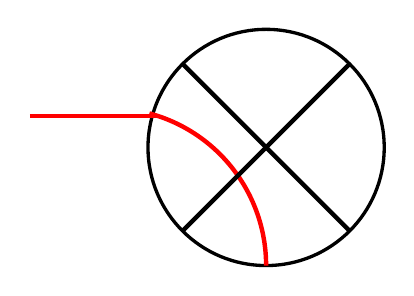
\begin{tikzpicture}
\filldraw[color=black,fill=none,very thick](-1,0) circle (1.5);
\draw[ultra thick, -,red] (-1,-1.5) arc (0:75:2);
\draw[ultra thick, red] (-4,0.4) -- (-2.4,0.4);
\draw[ultra thick, black] (0.06,1.06) -- (-2.06,-1.06);
\draw[ultra thick, black] (-2.06,1.06) -- (0.06,-1.06);

\end{tikzpicture}\\
\\
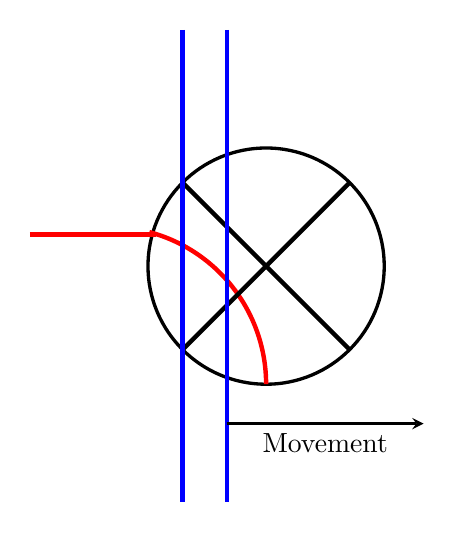
\begin{tikzpicture}
\tikzstyle{arrow} = [thick,->,>=stealth]
\filldraw[color=black,fill=none,very thick](-1,0) circle (1.5);
\draw[ultra thick, -,red] (-1,-1.5) arc (0:75:2);
\draw[ultra thick, red] (-4,0.4) -- (-2.4,0.4);
\draw[ultra thick, black] (0.06,1.06) -- (-2.06,-1.06);
\draw[ultra thick, black] (-2.06,1.06) -- (0.06,-1.06);


\draw[ultra thick, blue] (-2.06,3) -- (-2.06,-3);
\draw[ultra thick, blue] (-1.5,3) -- (-1.5,-3);

\draw [arrow] (-1.5,-2) -- node[anchor=north] {Movement} (1,-2);
\end{tikzpicture}
\newpage
\section{The laws of electromagnetic induction}
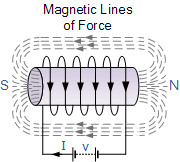
\includegraphics[width=5cm]{magnetic_induction.jpg}\\
North Pole - Anticlockwise current flow\\
South Pole - Clockwise current flow\\
\section{Lenz's law}
The direction of the induced emf is always such as to oppose the change that is causing it.\\
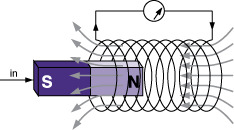
\includegraphics[width=5cm]{lenz.jpg}\\
As the magnet is pushed into the coil it induces an emf in the coil, this produces a magnetic field which opposes the potion. When removing the magnet the polarity will be inversed.\\
\section{Faraday's law}
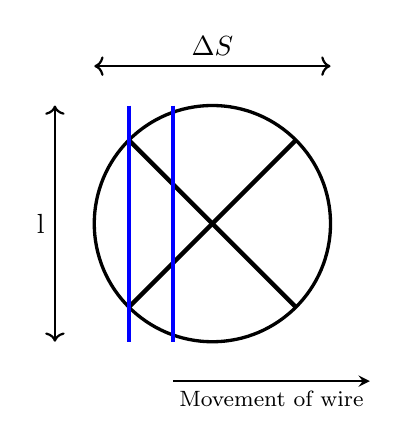
\begin{tikzpicture}
\tikzstyle{arrow} = [thick,->,>=stealth]
\filldraw[color=black,fill=none,very thick](-1,0) circle (1.5);

\draw[ultra thick, black] (0.06,1.06) -- (-2.06,-1.06);
\draw[ultra thick, black] (-2.06,1.06) -- (0.06,-1.06);


\draw[ultra thick, blue] (-2.06,1.5) -- (-2.06,-1.5);
\draw[ultra thick, blue] (-1.5,1.5) -- (-1.5,-1.5);

\draw [arrow] (-1.5,-2) -- node[anchor=north] {\footnotesize{Movement of wire}} (1,-2);
\draw[thick, <->] (-3,-1.5) -- (-3,1.5) node[anchor=east,midway] {l};

\draw[thick, <->] (-2.5,2) -- (0.5,2) node[anchor=south,midway] {$\Delta S$};
\end{tikzpicture}\\
\\
\begin{tabular}{r l}
Work done&$=F\times S$\\
&$=BIl\times\Delta S$
\end{tabular}\\
\\
Charge transfer, $Q=I\times\Delta t$\\
\\
$\epsilon=\dfrac{\text{Work done}}{\text{Charge}}=\dfrac{BIl\times\Delta S}{I\times\Delta t}=\dfrac{BA}{\Delta t}$\\
\\
\textcolor{red}{B=Magnetic flux density=$\dfrac{\phi}{A}$}\\
\textcolor{red}{$\phi$ = Magnetic flux}
$$\epsilon=\dfrac{\phi}{\Delta t}$$
\newpage
Faraday's law of electromagnetic induction is equal to the rate of change of flux(linkage) through the circuit.\\
\\
Flux linkage refers to coils, $N\phi$ replaces $\phi$ where N is the number of coils.
$$\epsilon=-N\dfrac{\Delta\phi}{\Delta t}$$
This equation may need to be expanded depending on the example
\subsection{Example}
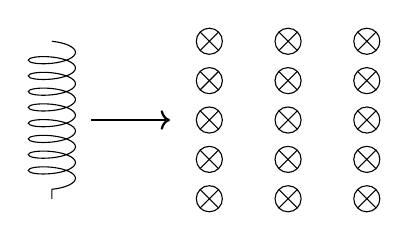
\begin{tikzpicture}[cross/.style={path picture={ 
  \draw[black]
(path picture bounding box.south east) -- (path picture bounding box.north west) (path picture bounding box.south west) -- (path picture bounding box.north east);
}},decoration={coil}]

 \node [draw,circle,cross,minimum width=2 mm] at (2,0){}; 
 \node [draw,circle,cross,minimum width=2 mm] at (2,-0.5){};
 \node [draw,circle,cross,minimum width=2 mm] at (2,-1){};
 \node [draw,circle,cross,minimum width=2 mm] at (2,-1.5){};
 \node [draw,circle,cross,minimum width=2 mm] at (2,-2){};
 
  \node [draw,circle,cross,minimum width=2 mm] at (3,0){}; 
 \node [draw,circle,cross,minimum width=2 mm] at (3,-0.5){};
 \node [draw,circle,cross,minimum width=2 mm] at (3,-1){};
 \node [draw,circle,cross,minimum width=2 mm] at (3,-1.5){};
 \node [draw,circle,cross,minimum width=2 mm] at (3,-2){};
 
   \node [draw,circle,cross,minimum width=2 mm] at (4,0){}; 
 \node [draw,circle,cross,minimum width=2 mm] at (4,-0.5){};
 \node [draw,circle,cross,minimum width=2 mm] at (4,-1){};
 \node [draw,circle,cross,minimum width=2 mm] at (4,-1.5){};
 \node [draw,circle,cross,minimum width=2 mm] at (4,-2){};
 
 \draw[decorate, decoration={aspect=0.3, segment length=2mm, amplitude=3mm}] (0,0) --(0,-2);
 
 \draw[thick, ->] (0.5,-1) -- (1.5,-1) ;
\end{tikzpicture}\\
\\
\textcolor{red}{$\epsilon=-N\dfrac{B\Delta A}{\Delta t}$}
\subsection{Magnets being dropped through a coil}
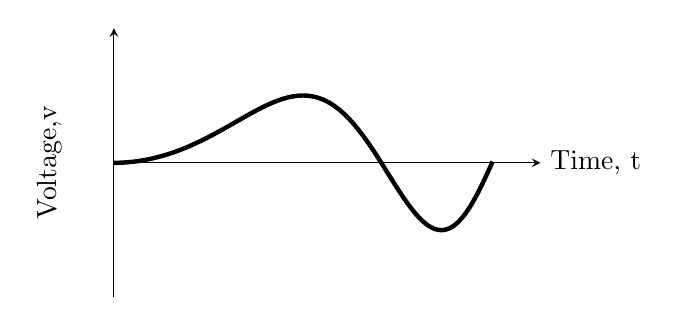
\begin{tikzpicture}
\begin{axis}[
    Axis Style,
    y label style={at={(axis description cs:-0.1,.5)},rotate=90,anchor=south},
    x label style={anchor=west},
    ylabel = {Voltage,v},
    xlabel= {Time, t},
    ticks=none
]
\addplot [mark=none, ultra thick, black,domain=0:3.55] {0.5*sin(deg(0.5*x^2))};
\end{axis}
\end{tikzpicture}
\\
\nth{1} peak - Wide, low\\
\nth{2} peak - High, narrow\\
\\
This is because the magnet accelerates, meaning the entry takes more time, and as it is travelling at a lower velocity on entry, the rate of flux cutting, and so the voltage is lower than the exit.
\section{EMF induced in a rotating coil}
$ $\\
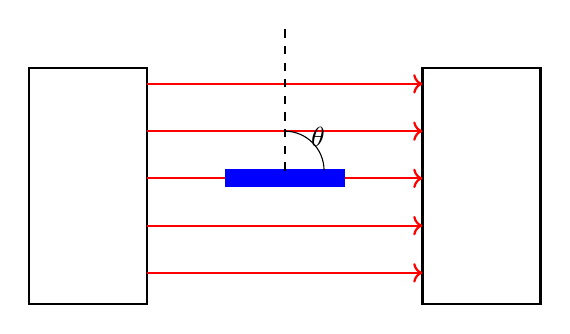
\begin{tikzpicture}
 
\draw[black,thick] (0,0)rectangle (1.5,3);
\draw[black,thick] (5,0)rectangle (6.5,3);
\draw[thick, ->,red] (1.5,2.8) -- (5,2.8);
\draw[thick, ->,red] (1.5,2.2) -- (5,2.2);
\draw[thick, ->,red] (1.5,1.6) -- (5,1.6);
\draw[thick, ->,red] (1.5,1) -- (5,1);
\draw[thick, ->,red] (1.5,0.4) -- (5,0.4);
\draw[blue,thick,fill=blue] (2.5,1.5)rectangle (4,1.7);
\draw [dashed,thick] (3.25,1.7) -- (3.25,3.5);
\coordinate (a) at (3.25,1.7);
\coordinate (b) at (3.25,2);
\coordinate (c) at (3.55,1.7);
\draw pic["$\theta$",draw=black,-,angle eccentricity=1.2,angle radius=0.5cm] {angle=c--a--b};
\end{tikzpicture}
\\
$\theta$ = The angle between the field lines and a line perpendicular to the coil\\
$$\textrm{Flux passing through the coil:} \ \phi=BA\cos\theta$$
$$\textrm{Flux linkage:} \ N\phi=BAN\cos\theta$$
\newpage
As the coil rotates the flux linkage varies\\
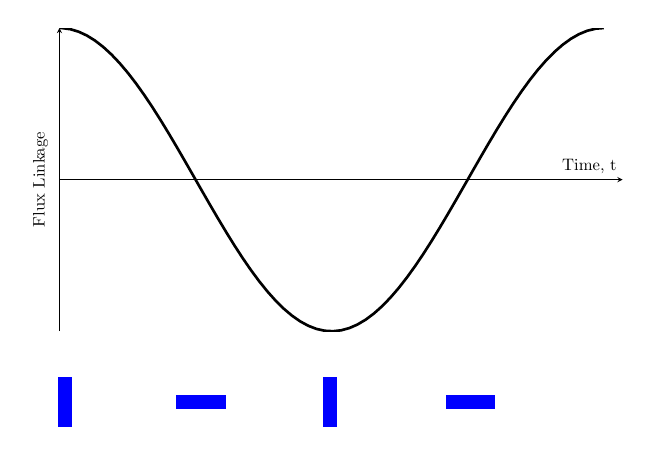
\begin{tikzpicture}[scale=0.6]
\begin{axis}[
    Axis Style 2,
    ticks=none,
    y label style={at={(axis description cs:-0.01,.5)},rotate=90,anchor=south},
    ylabel = {Flux Linkage},
    xlabel= {Time, t}
]
\addplot [mark=none, ultra thick, black] {cos(deg(x))};
\end{axis}
\draw[blue,thick,fill=blue] (0,-2)rectangle (0.25,-1);
\draw[blue,thick,fill=blue] (2.5,-1.625)rectangle (3.5,-1.375);
\draw[blue,thick,fill=blue] (5.6,-2)rectangle (5.85,-1);
\draw[blue,thick,fill=blue] (8.2,-1.625)rectangle (9.2,-1.375);
\end{tikzpicture}
\\
\\
\\
The speed that $\theta$ changes depends on angular velocity, $\omega$
$$\theta=\omega t$$
$$N\phi=BAN\cos(\omega t)$$
\\
EMF = Negative Rate of change of flux linkage\\
$$-\frac{d}{dt}BAN\cos(\omega t)=BAN\omega\sin(\omega t)$$
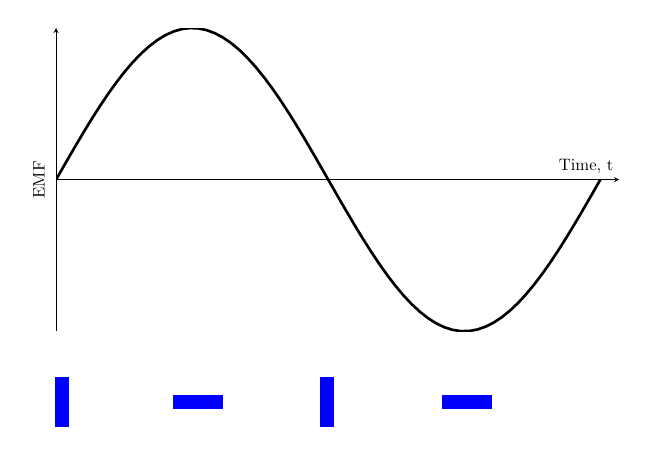
\begin{tikzpicture}[scale=0.6]
\begin{axis}[
    Axis Style 2,
    ticks=none,
    y label style={at={(axis description cs:-0.01,.5)},rotate=90,anchor=south},
    ylabel = {EMF},
    xlabel= {Time, t}
]
\addplot [mark=none, ultra thick, black] {sin(deg(x))};
\end{axis}
\draw[blue,thick,fill=blue] (0,-2)rectangle (0.25,-1);
\draw[blue,thick,fill=blue] (2.5,-1.625)rectangle (3.5,-1.375);
\draw[blue,thick,fill=blue] (5.6,-2)rectangle (5.85,-1);
\draw[blue,thick,fill=blue] (8.2,-1.625)rectangle (9.2,-1.375);
\end{tikzpicture}
\newpage
\subsection{Generators}
These effects can be used to create generators
\begin{figure}[h!]
    \centering
    \begin{minipage}{0.45\textwidth}
        \centering
        
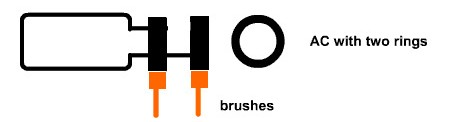
\includegraphics[width=7cm] {AC_Generator.jpg}  
\caption{AC Generator}    
    \end{minipage}\hfill
    \begin{minipage}{0.45\textwidth}
        \centering
        
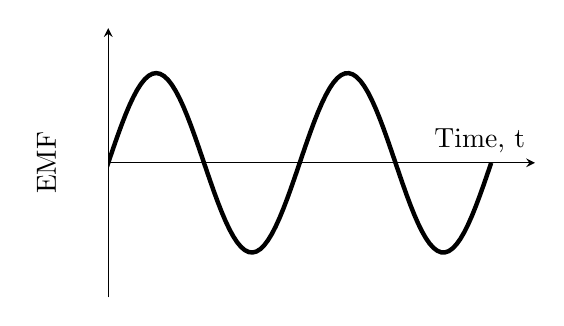
\begin{tikzpicture}
\begin{axis}[
    Axis Style 3,
    ticks=none,
    y label style={at={(axis description cs:-0.1,.5)},rotate=90,anchor=south},
    ylabel = {EMF},
    xlabel= {Time, t}
]
\addplot [mark=none, ultra thick, black] {sin(deg(x))};
\end{axis}
\end{tikzpicture}
\caption{Graph of EMF from an AC generator}

    \end{minipage}
\end{figure}

\begin{figure}[h]
    \centering
    \begin{minipage}{0.45\textwidth}
        \centering
        
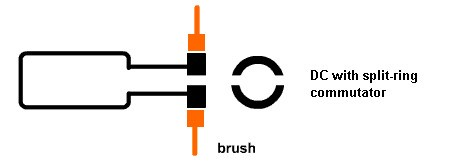
\includegraphics[width=7cm] {DC_Generator.jpg}  
\caption{DC Generator}    
    \end{minipage}\hfill
    \begin{minipage}{0.45\textwidth}
        \centering
        
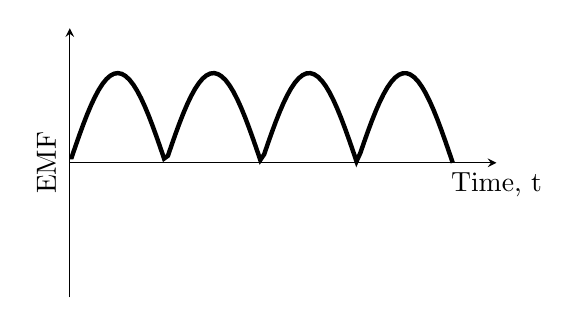
\begin{tikzpicture}
\begin{axis}[
    Axis Style 3,
    ticks=none,
    y label style={at={(axis description cs:-0.1,.5)},rotate=90,anchor=north},
    x label style={anchor=north},
    ylabel = {EMF},
    xlabel= {Time, t}
]
\addplot [mark=none, ultra thick, black] {abs(sin(deg(x)))};
\end{axis}
\end{tikzpicture}
\caption{Graph of EMF from a DC generator}

    \end{minipage}
\end{figure}
\newpage
\section{Transformers}
\subsection{Structure}
\begin{center}
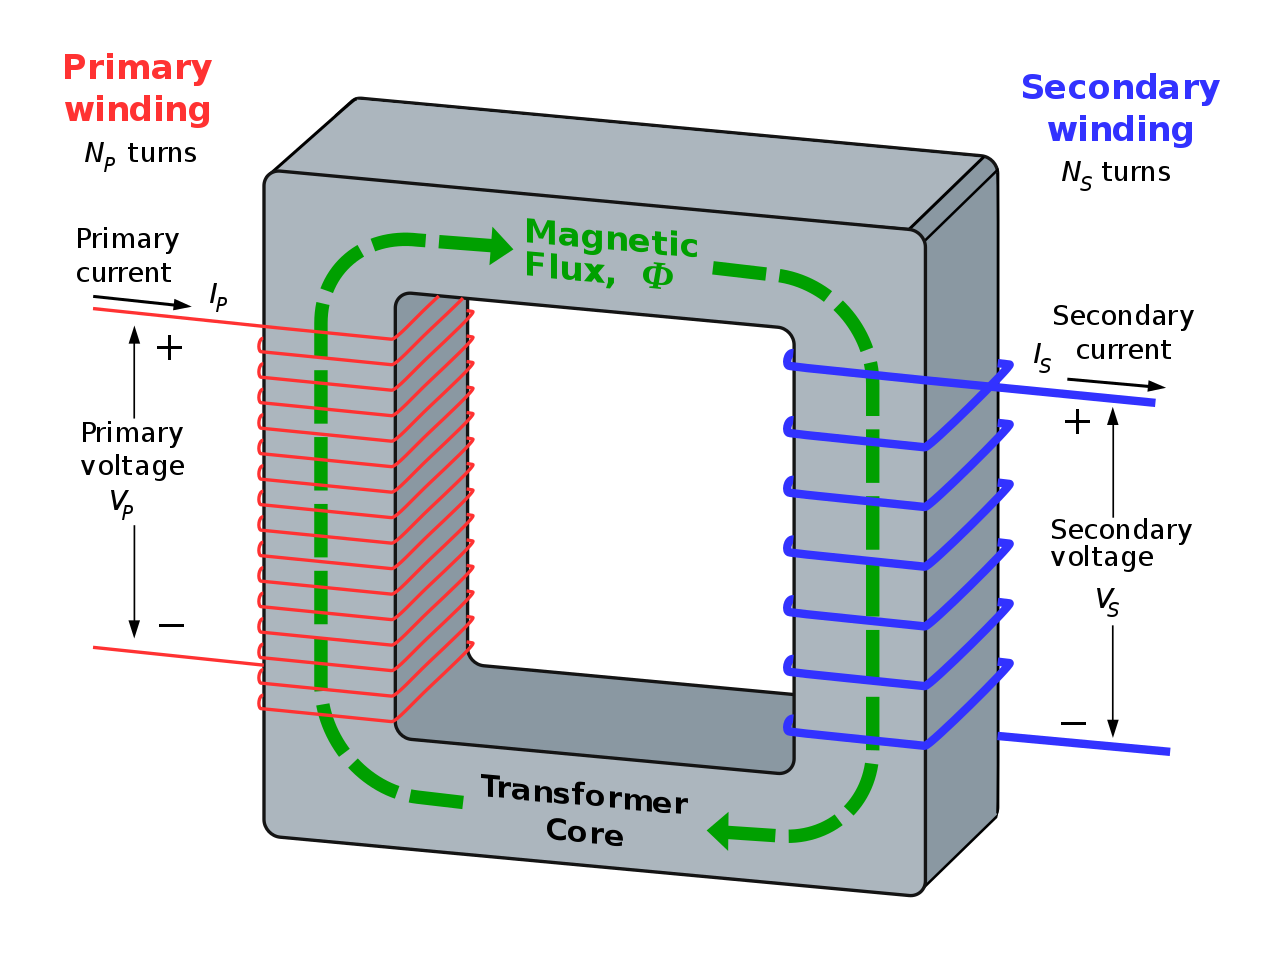
\includegraphics[width=8cm] {transformer.png}  
\end{center}
\subsection{What they are designed to do}
Increase or decrease an A.C. voltage\\
Step up - Increase\\
Step down - Decrease
\subsection{How they work}
\begin{itemize}
\item Two coils, primary and secondary, connected by a soft iron core
\item The primary coil is connected to a source of alternating p.d., creating an alternating magnetic field in the core
\item The field passes through the secondary coil, creating an alternating emf in the secondary coil
\item A transformer is designed so all the magnetic flux produced by the primary coil passes through the secondary coil
\end{itemize}
\subsection{How energy losses are reduced}
\begin{enumerate}
\item Low resistance windings to reduce power wasted due to the heating effect of the current
\item A laminated core which consists of layers of iron separated by layers of insulator. Induced currents in the core itself, referred to as \textbf{eddy currents}, are reduced in this was so the magnetic flux is as high as possible. Also, the heating effect of the induced currents in the core are reduced
\item A core of \textbf{soft iron} which is easily magnetised and demagnetised. This reduces power wasted through repeated magnetisation and demagnetisation of the core
\end{enumerate}  
\subsection{Equations}
$$\frac{V_P}{V_S}=\frac{N_P}{N_S}=\frac{I_S}{I_P}$$
$$\textrm{Efficiency}=\frac{I_SV_S}{I_PV_P}\times100$$
\newpage
\section{The national grid}
Transmission of electrical power over long distances is much more efficient at high voltages compared to low voltages.
\subsection{Transmit 1MW of power through wires of resistance $500\Omega$}
\subsubsection{At 25kV}
$$I=\frac{P}{V}=\frac{1\times10^6}{25\times10^3}=40A$$
$$\textrm{Power lost as heat}=I^2R=40^2\times500=0.8MW=20\%  \ \textrm{Efficient}$$
\subsubsection{At 400kV}
$$I=\frac{P}{V}=\frac{1\times10^6}{400\times10^3}=2.5A$$
$$\textrm{Power lost as heat}=I^2R=2.5^2\times500=0.003MW=99.7\%  \ \textrm{Efficient}$$

\end{document}